\subsection*{Problema 01}

\noindent\textbf{Enunciado:} \\
Calcular la integral indefinida:
\begin{equation*}
\int \frac{dx}{1 + \sin x + \cos x}
\end{equation*}

\noindent\textbf{Solución:} \\
Para resolver esta integral trigonométrica, utilizamos la sustitución universal de Weierstrass:
\begin{align*}
z &= \tan\left(\frac{x}{2}\right), \quad dx = \frac{2 \, dz}{1 + z^2} \\
\sin x &= \frac{2z}{1 + z^2}, \quad \cos x = \frac{1 - z^2}{1 + z^2}
\end{align*}

\noindent
Sustituimos estas expresiones en la integral original:
\begin{align*}
I &= \int \frac{\frac{2 \, dz}{1 + z^2}}{1 + \frac{2z}{1 + z^2} + \frac{1 - z^2}{1 + z^2}}
\end{align*}

\noindent
Simplificamos el denominador multiplicando toda la fracción por $(1 + z^2)$:
\begin{align*}
I &= \int \frac{2 \, dz}{(1 + z^2) + 2z + (1 - z^2)} \\
I &= \int \frac{2 \, dz}{2 + 2z} = \int \frac{dz}{1 + z}
\end{align*}

\noindent
La integral resultante es inmediata y se resuelve mediante un cambio de variable logarítmico:
\begin{align*}
I &= \ln|1 + z| + C
\end{align*}

\noindent
Finalmente, regresamos a la variable original $x$ sustituyendo $z = \tan(x/2)$:
\begin{align*}
I &= \ln\left|1 + \tan\left(\frac{x}{2}\right)\right| + C
\end{align*}

\begin{figure}[H]
	\centering
	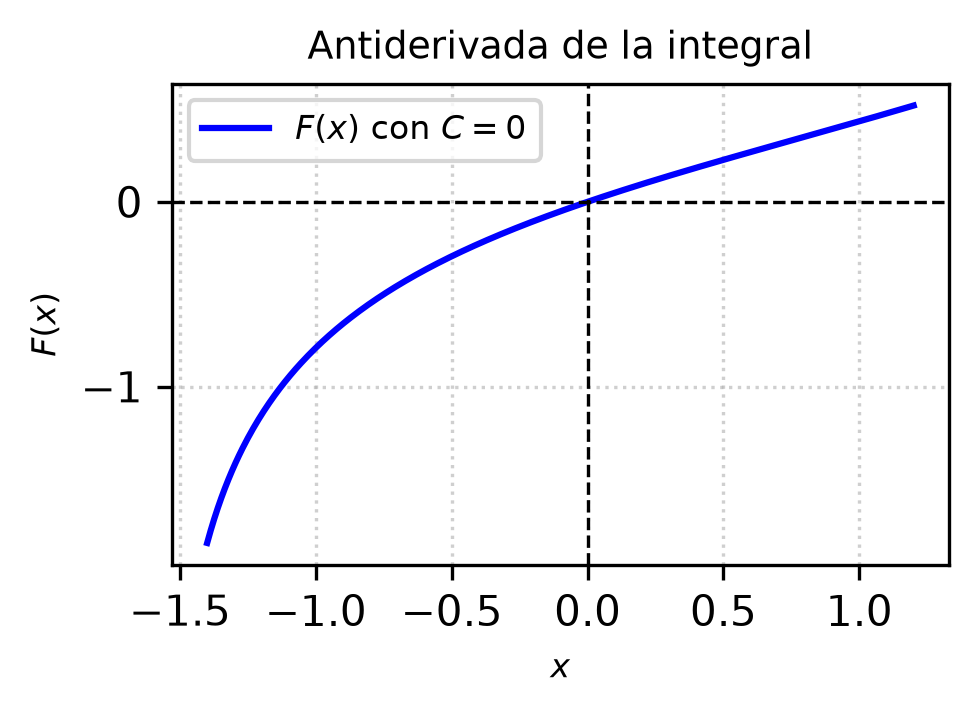
\includegraphics[width=\columnwidth]{semana_04/graficas/SEM04_P01_grafica.png}
	\caption{Representación gráfica de $f(x)$ y su antiderivada $F(x)$ evaluada para la constante de integración $C = 0$ (Problema 01).}
	\label{fig:problema01}
\end{figure}
